\chapter{Introducción}\label{chapter\:introduction}

\section{Motivación}
\textit{Gaussian Splatting (GS)} [\cite{kerbl20233d}] se ha consolidado recientemente como uno de los métodos más efectivos para la representación y 
visualización eficiente de escenas tridimensionales. La relevancia del GS se evidencia en la adopción generalizada 
de este framework en trabajos recientes que abordan desde reconstrucciones dinámicas en cuatro dimensiones hasta representaciones volumétricas complejas. 
Sin embargo, a pesar de sus ventajas, GS presenta limitaciones importantes relacionadas con la forma subóptima adoptada por las gaussianas durante el 
entrenamiento. Diversos estudios han demostrado que estas gaussianas tienden a degenerar en formas anisotrópicas dominadas por una sola varianza, 
lo que genera artefactos en forma de aguja, geometrías subóptimas y normales inexactas [\cite{hyung2024effectiverankanalysisregularization, huang2024spectralgstaming3dgaussian,yu2023mipsplattingaliasfree3dgaussian}]. 
Asimismo, otro problema fundamental surge de la incapacidad inherente del GS para modelar adecuadamente discontinuidades y límites definidos 
debido a la naturaleza continua de las distribuciones gaussianas [\cite{qu2024discgsdiscontinuityawaregaussiansplatting}]. Por tanto, surge 
la necesidad de investigar nuevas alternativas para mejorar estas limitaciones sin afectar significativamente la estructura general del método
para que pueda ser adaptado a otras investigaciones ya existentes.

\section{Problemática}
La técnica de \textit{Gaussian Splatting} ha demostrado ser una herramienta poderosa para la representación de escenas tridimensionales complejas,
sin embargo, a pesar de su eficacia general, se han identificado una serie de limitaciones fundamentales que comprometen su rendimiento 
en escenarios reales, especialmente en aquellos donde se requiere una alta fidelidad en los detalles geométricos y visuales.

Una de las principales problemáticas asociadas al \textit{Gaussian Splatting} es la tendencia de las gaussianas a adquirir formas altamente anisotrópicas 
durante el proceso de optimización. Esto significa que, en lugar de mantener una forma más esférica o moderadamente elipsoidal, las gaussianas 
tienden a elongarse excesivamente en una dirección específica, generando artefactos visuales conocidos como agujas. 
Este comportamiento, reportado en estudios recientes  [\cite{hyung2024effectiverankanalysisregularization, huang2024spectralgstaming3dgaussian, yu2023mipsplattingaliasfree3dgaussian}],
no solo degrada la calidad visual de la reconstrucción, sino que también compromete la precisión de las normales estimadas, lo cual es crítico 
en tareas de iluminación realista y renderizado de alta calidad.

Además de esta degeneración geométrica, existe otra limitación importante: la incapacidad inherente del modelo para representar adecuadamente 
bordes abruptos, discontinuidades o superficies con cambios de curvatura pronunciados. Esta deficiencia proviene del hecho de que las gaussianas 
son distribuciones continuas por naturaleza, lo que las hace poco adecuadas para capturar transiciones bruscas en los datos visuales. Este fenómeno 
ha sido discutido en trabajos como \cite{qu2024discgsdiscontinuityawaregaussiansplatting}, donde se señala explícitamente que el 
uso exclusivo de gaussianas limita la capacidad del modelo para representar bordes definidos, afectando negativamente la reconstrucción 
de objetos con geometría compleja o detalles finos.

Cabe señalar que estas limitaciones no solo afectan la calidad visual, sino que también restringen la aplicabilidad del \textit{Gaussian Splatting} en 
contextos más exigentes, como reconstrucciones en tiempo real, modelado de escenas dinámicas, o aplicaciones donde la precisión geométrica es 
un factor determinante. En muchos casos, estas deficiencias obligan a recurrir a soluciones alternativas o a incorporar etapas adicionales de 
postprocesamiento que aumentan la complejidad y el costo computacional del sistema.

Por tanto, abordar esta problemática no es solo una cuestión de mejora estética o cuantitativa, sino una necesidad crítica para extender la 
utilidad práctica del \textit{Gaussian Splatting} a un espectro más amplio de aplicaciones. Resolver el problema de la forma subóptima de las gaussianas 
y su limitada capacidad de representación abre la puerta a métodos más robustos, adaptables y precisos.

\section{Antecedentes}
Existen diversas aproximaciones que han intentado resolver o mitigar las limitaciones mencionadas mediante modificaciones en la estructura 
fundamental de la gaussiana empleada en GS 
[\cite{qu2024discgsdiscontinuityawaregaussiansplatting, li20243d, huang2025deformableradialkernelsplatting,held20243dconvexsplattingradiance}]. 
Estas modificaciones buscan adaptar la forma, orientación o dispersión de las gaussianas para capturar mejor la complejidad geométrica de las escenas. 
No obstante, muchas de estas soluciones implican alteraciones significativas al pipeline original o introducen parámetros adicionales que aumentan la 
complejidad computacional y la demanda de memoria. 
Por esta razón, encontrar una solución que combine eficiencia computacional con mejoras sustanciales en la calidad visual y que a la vez sea adaptable 
a investigaciones realizadas sobre el \textit{Gaussian Splatting} original, sigue siendo un desafío relevante.

\section{Objetivos}
El objetivo general de esta investigación es mejorar la calidad visual y precisión geométrica del método de \textit{Gaussian Splatting} mediante la 
introducción y evaluación de un nuevo parámetro basado en la asimetría o \textit{skewness}. Los objetivos específicos incluyen:
\begin{itemize}
    \item Evaluar el impacto del parámetro de asimetría en la calidad visual mediante métricas estándar utilizadas en datasets comúnmente empleados.
    \item Mantener un bajo costo computacional y un consumo de memoria moderado, garantizando un rendimiento en términos de fotogramas por segundo (FPS) 
    similar o ligeramente inferior al del método original.
    \item Proporcionar una metodología clara y eficiente para la integración del nuevo parámetro dentro del pipeline existente del GS.
\end{itemize}

\section{Propuestas de Solución}
La propuesta central de esta tesis consiste en incorporar un nuevo conjunto de parámetros que permitan añadir complejidad visual a la escena sin añadir
mucho coste computacional. Debido a que al \textit{Gaussian Splatting} le cuesta representar discontinuidades tales como bordes de objetos o cambios
de color bruscos [\cite{qu2024discgsdiscontinuityawaregaussiansplatting}] y por ello tiende a crear gaussianas con formas de aguja para suplir esta carencia
[\cite{hyung2024effectiverankanalysisregularization, huang2024spectralgstaming3dgaussian,yu2023mipsplattingaliasfree3dgaussian}], hacer que las gaussianas posean bordes duros en una dirección entrenable podría resolver esta problemática.    
La asimetría o \textit{skewness} cumple las condiciones necesarias, por ello en este trabajo se busca simularla en la distribución de las 
gaussianas tridimensionales utilizadas. Concretamente, se proponen cuatro nuevos parámetros: $s_x, s_y, s_z$ para definir 
la dirección y magnitud del desplazamiento en tres dimensiones de una segunda gaussiana idéntica a la original, y un parámetro adicional $S$, que 
controla la intensidad del efecto de asimetría. Esta modificación es implementada mediante la función:

\begin{equation}
    A \cdot (1-e^{-S \cdot B})
\end{equation}    

donde $B$ representa la gaussiana original $A$ desplazada por los parametros $s_x, s_y, s_z$ . La elección de esta aproximación radica en su capacidad 
para introducir un corportamiento parecido a la asimetría sin modificar sustancialmente el algoritmo original de rasterización diferenciable.

\begin{figure}[htbp]
    \centering
    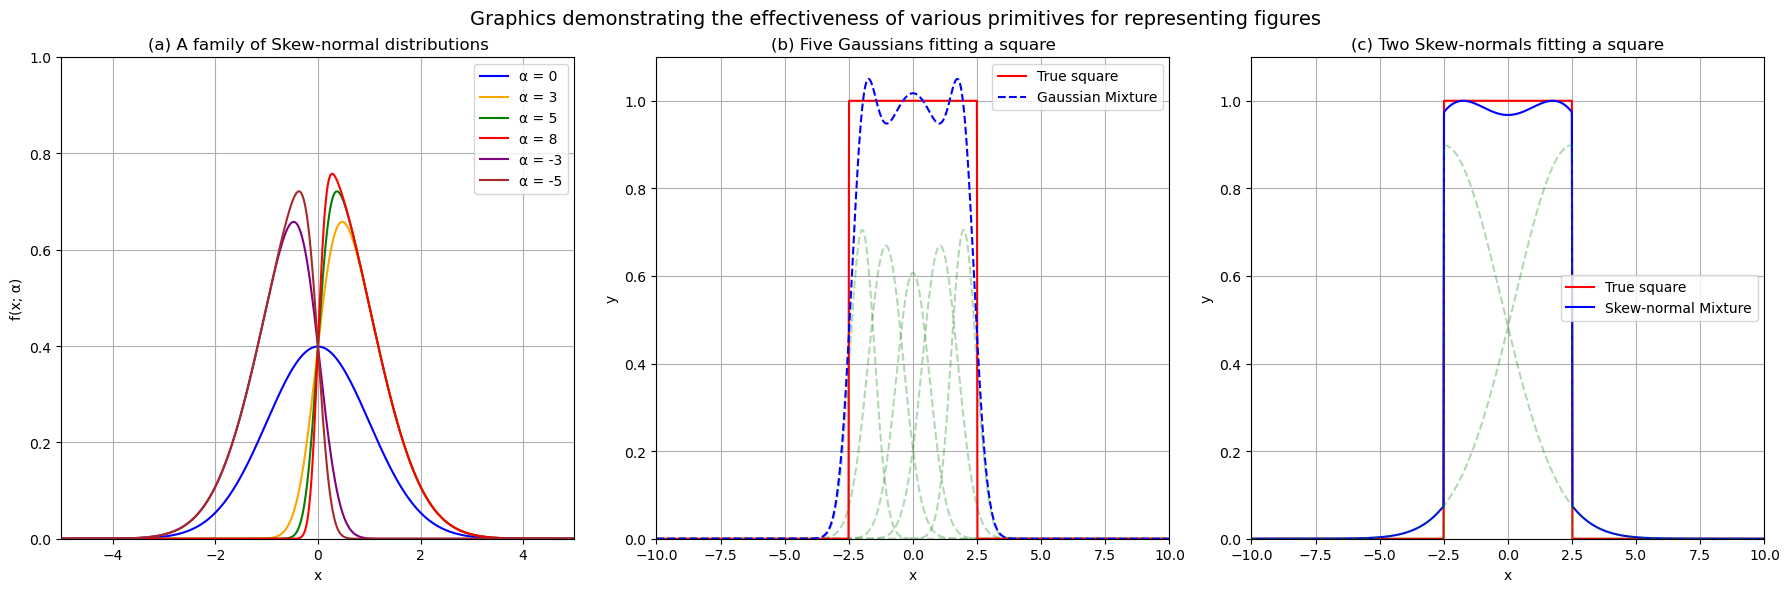
\includegraphics[width=1\textwidth]{Graphics/square.png}
    \caption{Función de distribución normal con asimetría. 
    (a): Se muestra una familia de distribuciones normales con asimetría \(f(x; \alpha)\) con diferentes valores de \(\alpha\), 
    para \(\mu = 0\), \(\sigma = 1\). Cuando \(\alpha = 0\), la función se reduce a la función gaussiana estándar. 
    En nuestro enfoque, aprendemos \(\alpha\) como otro parámetro de cada componente. 
    (b,c): La superposición de normales con asimetría, con \(\alpha\) entrenable, 
    se ajusta la misma señal (cuadrada) con menos componentes en comparación con funciones gaussianas utilizando optimización basada en gradientes. 
    (b): Se muestra un ejemplo de la superposición de normales ajustada con \(N = 5\) componentes vs. 
    (c) cuando se usa la distribución normal con asimetría con \(N = 2\) componentes. La distribución normal con asimetría logra una menor pérdida de error y 
    aproxima mejor los bordes pronunciados que la versión gaussiana, utilizando menos componentes. Los componentes individuales optimizados 
    (inicializados con parámetros aleatorios) se muestran en verde después de la convergencia.}
    \label{fig:square}
\end{figure}    

\section{Estructura de la Tesis}
La tesis se organiza en los siguientes capítulos:
\begin{itemize}
    \item \textbf{Capítulo 2: Marco Teórico.} Se presentan conceptos fundamentales sobre espacios gaussianos, proyección y rasterización diferenciable, 
    y propiedades de distribuciones sesgadas.
    \item \textbf{Capítulo 3: Estado del Arte.} Se realiza una revisión crítica de \textit{Gaussian Splatting} y otros métodos relacionados, incluyendo técnicas 
    previas que abordan la modificación de las primitivas geométricas.
    \item \textbf{Capítulo 4: Metodología Propuesta.} Se detallan los aspectos teóricos y prácticos de la solución propuesta, incluyendo la simulación 
    de la asimetría y análisis de complejidad computacional.
    \item \textbf{Capítulo 5: Detalles de Implementación.} Se describen los componentes principales del código, incluyendo kernels forward y backward 
    utilizados en el algoritmo de rasterización diferenciable propuesto.
    \item \textbf{Capítulo 6: Experimentos.} Se presentan hipótesis, diseño experimental, métricas de evaluación y resultados obtenidos tanto cuantitativos 
    como cualitativos.
    \item \textbf{Conclusiones y Recomendaciones.} Se resumen los aportes principales, limitaciones, aplicaciones potenciales y líneas futuras de 
    investigación sugeridas.
\end{itemize}
